\label{sec:intro}

The models for computing the orbits for Sag are summarized in table 1.

\begin{table}[H]
\begin{center}
\begin{tabular}{c c c c c}
\hline
\textbf{MW} & Model & Mass [$M_{\odot}$] &  & \\
\hline
DM halo & NFW & $M_{vir} = 1E12$ &$R_{vir} = 261$ &  $r_s = 26.47$ \\
Disk & Miyamoto-Nagai &  $M_d = 6.5E10$ & $r_a = 3.5$ &  $r_b=0.53$  \\
Bulge & Hernquist &  $M_b = 1E10$  & $r_{h} = 26.47 $ &   \\
\hline
\textbf{Sag} & & & &  \\
\hline
DM halo heavy& NFW & $M = 1E11 $ & $r_s=6.5$ & $r_{vir} = 121.25 kpc$ \\
DM halo light & NFW & $M=0.32E11 $ & $r_s = 4.9$ & $r_{vir} = 82.93 kpc$ \\
\hline
\end{tabular}
\end{center}
\caption{}
\end{table}

Fig. 1 shows the orbits of Sag for the heavy N-body sag, and the light 
and heavy analytical integration. The IC for the analytical integration
(both light and heavy) where the first positions and velocities of 
the N-body orbit.  

\begin{figure}[H]
\centering
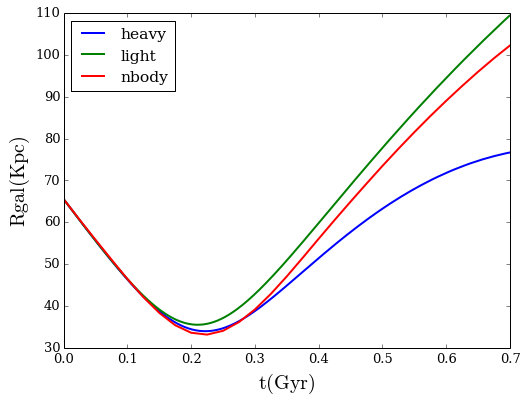
\includegraphics[scale=0.7]{facundo_plot_sag.png}
\caption{}
\end{figure}


To correct the orbit the dynamical friction equation is modified 
with an $\alpha$ parameter as follows:

\begin{equation}
a_{df} = -4\pi G^2 M_{sat} \rho \alpha Ln(\Lambda)  \left( erf(X) - \dfrac{2X}{\sqrt{\pi}}exp(-X^2)   \right) \vec{v}/v^3
\end{equation}

\begin{figure}[H]
\centering
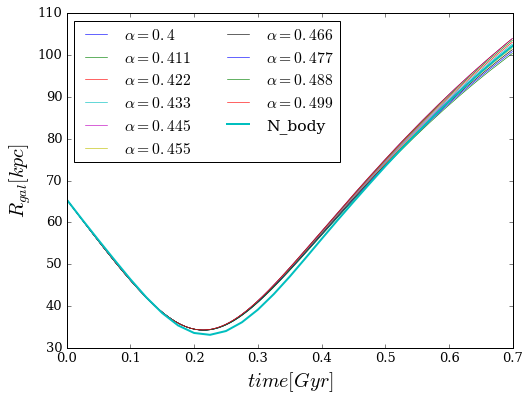
\includegraphics[scale=0.7]{../orbits_comparison_pos.png}
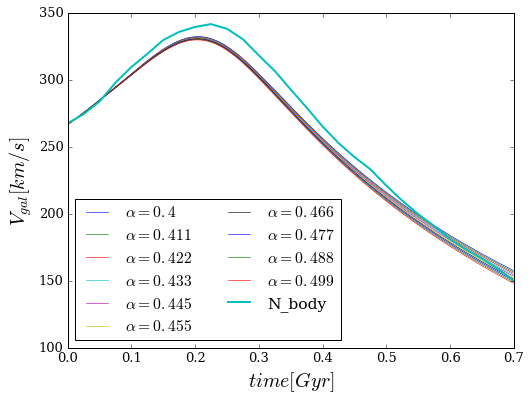
\includegraphics[scale=0.7]{../orbits_comparison_vel.png}
\caption{}
\end{figure}

The orbits for different $\alpha$ are shown in Fig.2, The best orbit (defined as the one
that ends closer in positions and velocities to the N-Body orbit) is for $\alpha=0.457$.
The final galatocentric position and velocity of the interated and N-body orbits 
are summarized in table 2.

\begin{table}[H]
\begin{tabular}{c c c c c c}
\hline
x(kpc) & y(kpc) & z(kpc) & vx(km/s) & vy(km/s)& vz(km/s) & 
\hline
N-body & & & & & \\
101.3 & 0.83 & -13.82 & 130.25 & -1.59 & 74.75 \\
Integration & & & & & \\
\hline
99.87 & 1.195 & -21.97 & 136.29 & 3.25 & 75.78 \\ 
\hline
\end{tabular}
\caption{}
\end{table}  	

With this $\alpha$ the Sagittarius orbit was integrated backwards in time starting
from the initial conditions provided by Purcell \& Bullock and 
with the galaxy models provided in Gomez et al. Fig. 3 shows
the orbits of the sagittarius dwarf galaxy for $\alpha=1$
and $\alpha=0.44$. The initial conditions at $R_{vir}=261 kpc$
are summarized in table 3.



\begin{figure}[H]
\centering
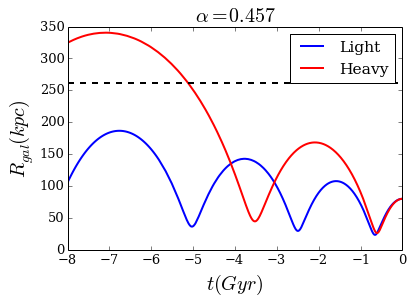
\includegraphics[scale=0.7]{sag_orbit_mdf.png}
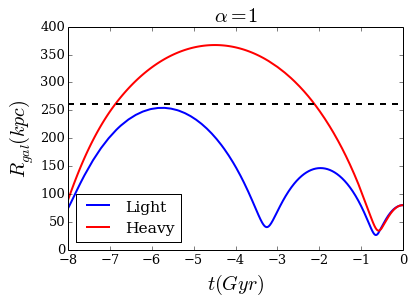
\includegraphics[scale=0.7]{sag_orbit.png}
\caption{}
\end{figure}

\begin{table}
\begin{tabular}{c c c c c c c}
\hline
Model & x(kpc) & y(kpc) & z(kpc) & vx(km/s) & vy(km/s) & vz(km/s) \\
\hline
${\alpha=1}$ & & & & & & \\
%ight Sag & -136.51 & 0 & 137.15 & 20.85 &  0 & -68.54  \\ 
%MW & 7.03 & 0 & -80.19 & 15.5 & 0 & 39.85 \\
%\hline
Heavy Sag & -146.23 & 0 & 145.26 & 25.06 & 0 & -78.83 \\
MW & 8.41 & 0 & -64.97 & 12.39  & 0 & 31.93\\
\hline
${\alpha=0.57}$ & & & & & & \\
%Light Sag & -215.79  & 0 & -241.19 & 80.4 & 0 & 17.8 \\ 
%MW & 9.93 & 0 & -110.18 & -10.03 & 0  & 33.68 \\
\hline
Heavy Sag & -206.66 & 0  & -231.59 & 95.05 & 0 & 23.5 \\
MW & 6.36 & 0 & -80.85 & -9.64 & 0 & 24.019\\
\hline
\end{tabular}
\caption{}
\end{table}

The projected orbits are shown in Fig. 4.

\begin{figure}[H]
\centering
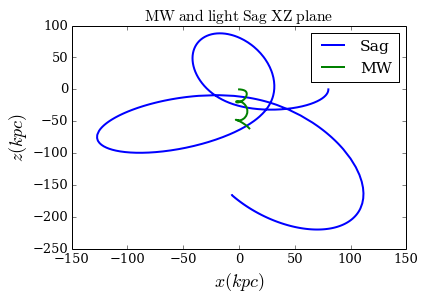
\includegraphics[scale=0.7]{MW_lsag_XZ.png}
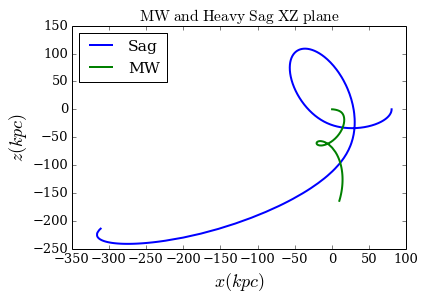
\includegraphics[scale=0.7]{MW_hsag_XZ.png}
\caption{}
\end{figure}
